% GNUPLOT: LaTeX picture with Postscript
\begingroup
  \makeatletter
  \providecommand\color[2][]{%
    \GenericError{(gnuplot) \space\space\space\@spaces}{%
      Package color not loaded in conjunction with
      terminal option `colourtext'%
    }{See the gnuplot documentation for explanation.%
    }{Either use 'blacktext' in gnuplot or load the package
      color.sty in LaTeX.}%
    \renewcommand\color[2][]{}%
  }%
  \providecommand\includegraphics[2][]{%
    \GenericError{(gnuplot) \space\space\space\@spaces}{%
      Package graphicx or graphics not loaded%
    }{See the gnuplot documentation for explanation.%
    }{The gnuplot epslatex terminal needs graphicx.sty or graphics.sty.}%
    \renewcommand\includegraphics[2][]{}%
  }%
  \providecommand\rotatebox[2]{#2}%
  \@ifundefined{ifGPcolor}{%
    \newif\ifGPcolor
    \GPcolortrue
  }{}%
  \@ifundefined{ifGPblacktext}{%
    \newif\ifGPblacktext
    \GPblacktextfalse
  }{}%
  % define a \g@addto@macro without @ in the name:
  \let\gplgaddtomacro\g@addto@macro
  % define empty templates for all commands taking text:
  \gdef\gplbacktext{}%
  \gdef\gplfronttext{}%
  \makeatother
  \ifGPblacktext
    % no textcolor at all
    \def\colorrgb#1{}%
    \def\colorgray#1{}%
  \else
    % gray or color?
    \ifGPcolor
      \def\colorrgb#1{\color[rgb]{#1}}%
      \def\colorgray#1{\color[gray]{#1}}%
      \expandafter\def\csname LTw\endcsname{\color{white}}%
      \expandafter\def\csname LTb\endcsname{\color{black}}%
      \expandafter\def\csname LTa\endcsname{\color{black}}%
      \expandafter\def\csname LT0\endcsname{\color[rgb]{1,0,0}}%
      \expandafter\def\csname LT1\endcsname{\color[rgb]{0,1,0}}%
      \expandafter\def\csname LT2\endcsname{\color[rgb]{0,0,1}}%
      \expandafter\def\csname LT3\endcsname{\color[rgb]{1,0,1}}%
      \expandafter\def\csname LT4\endcsname{\color[rgb]{0,1,1}}%
      \expandafter\def\csname LT5\endcsname{\color[rgb]{1,1,0}}%
      \expandafter\def\csname LT6\endcsname{\color[rgb]{0,0,0}}%
      \expandafter\def\csname LT7\endcsname{\color[rgb]{1,0.3,0}}%
      \expandafter\def\csname LT8\endcsname{\color[rgb]{0.5,0.5,0.5}}%
    \else
      % gray
      \def\colorrgb#1{\color{black}}%
      \def\colorgray#1{\color[gray]{#1}}%
      \expandafter\def\csname LTw\endcsname{\color{white}}%
      \expandafter\def\csname LTb\endcsname{\color{black}}%
      \expandafter\def\csname LTa\endcsname{\color{black}}%
      \expandafter\def\csname LT0\endcsname{\color{black}}%
      \expandafter\def\csname LT1\endcsname{\color{black}}%
      \expandafter\def\csname LT2\endcsname{\color{black}}%
      \expandafter\def\csname LT3\endcsname{\color{black}}%
      \expandafter\def\csname LT4\endcsname{\color{black}}%
      \expandafter\def\csname LT5\endcsname{\color{black}}%
      \expandafter\def\csname LT6\endcsname{\color{black}}%
      \expandafter\def\csname LT7\endcsname{\color{black}}%
      \expandafter\def\csname LT8\endcsname{\color{black}}%
    \fi
  \fi
  \setlength{\unitlength}{0.0500bp}%
  \begin{picture}(5668.00,4534.00)%
    \gplgaddtomacro\gplbacktext{%
      \csname LTb\endcsname%
      \put(264,2050){\makebox(0,0)[r]{\strut{} 300}}%
      \csname LTb\endcsname%
      \put(264,2631){\makebox(0,0)[r]{\strut{} 400}}%
      \csname LTb\endcsname%
      \put(264,3211){\makebox(0,0)[r]{\strut{} 500}}%
      \csname LTb\endcsname%
      \put(264,3792){\makebox(0,0)[r]{\strut{} 600}}%
      \csname LTb\endcsname%
      \put(264,4372){\makebox(0,0)[r]{\strut{} 700}}%
      \csname LTb\endcsname%
      \put(618,1366){\makebox(0,0){\strut{}}}%
      \csname LTb\endcsname%
      \put(1726,1366){\makebox(0,0){\strut{}}}%
      \csname LTb\endcsname%
      \put(2834,1366){\makebox(0,0){\strut{}}}%
      \csname LTb\endcsname%
      \put(3941,1366){\makebox(0,0){\strut{}}}%
      \csname LTb\endcsname%
      \put(5049,1366){\makebox(0,0){\strut{}}}%
      \put(-242,3037){\rotatebox{-270}{\makebox(0,0){\strut{}Radius size / pixel}}}%
    }%
    \gplgaddtomacro\gplfronttext{%
      \csname LTb\endcsname%
      \put(1314,3682){\makebox(0,0)[r]{\strut{}AgBehe}}%
      \csname LTb\endcsname%
      \put(1314,3462){\makebox(0,0)[r]{\strut{}SBA}}%
    }%
    \gplgaddtomacro\gplbacktext{%
      \csname LTb\endcsname%
      \put(264,558){\makebox(0,0)[r]{\strut{}-3}}%
      \csname LTb\endcsname%
      \put(264,768){\makebox(0,0)[r]{\strut{}-2}}%
      \csname LTb\endcsname%
      \put(264,978){\makebox(0,0)[r]{\strut{}-1}}%
      \csname LTb\endcsname%
      \put(264,1188){\makebox(0,0)[r]{\strut{} 0}}%
      \csname LTb\endcsname%
      \put(264,1398){\makebox(0,0)[r]{\strut{} 1}}%
      \csname LTb\endcsname%
      \put(618,233){\makebox(0,0){\strut{}2500}}%
      \csname LTb\endcsname%
      \put(1726,233){\makebox(0,0){\strut{}3000}}%
      \csname LTb\endcsname%
      \put(2834,233){\makebox(0,0){\strut{}3500}}%
      \csname LTb\endcsname%
      \put(3941,233){\makebox(0,0){\strut{}4000}}%
      \csname LTb\endcsname%
      \put(5049,233){\makebox(0,0){\strut{}4500}}%
      \put(22,1020){\rotatebox{-270}{\makebox(0,0){\strut{}Residuals / pixel}}}%
      \put(2833,-97){\makebox(0,0){\strut{}Measured distance / mm}}%
    }%
    \gplgaddtomacro\gplfronttext{%
    }%
    \gplbacktext
    \put(0,0){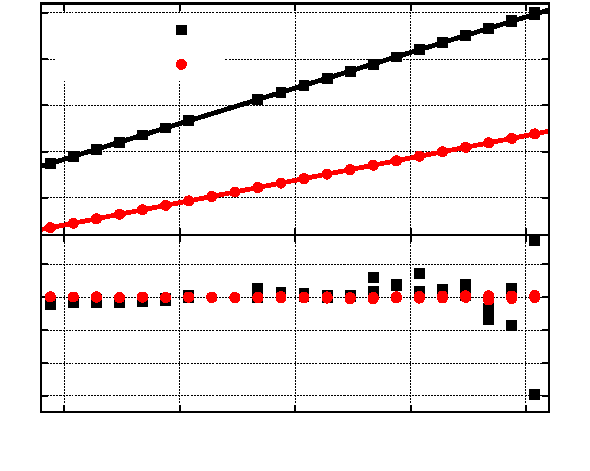
\includegraphics{DistanceCalibrationSAXS}}%
    \gplfronttext
  \end{picture}%
\endgroup
